\section{Introduction}
\todo{write about paper content - challenging for technology harsh environment and cultural acceptance - very conservative - in this paper we describe the conweardi project, an approach to overcome these challenges and propose a method and vision for digitazing constructions.}
Construction projects can vary in size and complexity... In our research, we focus on smaller constructions like house construction (compared to large civil engineering projects), where the work on one site is accomplished mostly by few on-site workers. Nonetheless, managing workflows and resources for such craftsman businesses can be very challenging.

\section{Problem description}
The construction industry shows a huge potential for digitization and it's still in the early phase of adopting technologies related to Industry 4.0. 
Meanwhile the Building Information Modeling (BIM) supports the processes of the design and planing phase, the actual construction, the execution process of the value creation, is still dominated by analog processes and paper documents. 
Examples include wall sized printed plans and time sheets on paper, which are only digitally recorded in the office and are available only there. 
So, in many cases, the digital world ends in the back office or the workstations of the architects and engineers. 
The potential of novel services, such as Internet of Things (IoT) systems with sensors and actuators deployed on site connecting it to powerful computing resources, remained untapped.

\section{Project goal}
Our main goal in the ConWearDi project is the design and prototype implementation of a platform capable to capture and analyze the current state of the construction work and to provide useful informational support not only for the managers and engineers but directly to the construction workers and craftsmen on site. 

%Information sources, which provide structured information and accurate specifications (e.g. used materials) about a project, such as the BIM itself, are the foundation to achieve this goal. These

The main project goals can be summarized as:
\begin{enumerate}
  \item Creation of a Digital Twin, a digital representation of the construction site, which always reflects it's current state in real time. 
  \item Centralized system for managing the construction site
  \item Automatic documentation for knowledge- and quality management purposes
  \item Exploration of new business models
  \item Development of methods for monitoring the activities of different worker groups with wearable technologies
\end{enumerate}


\begin{figure*}
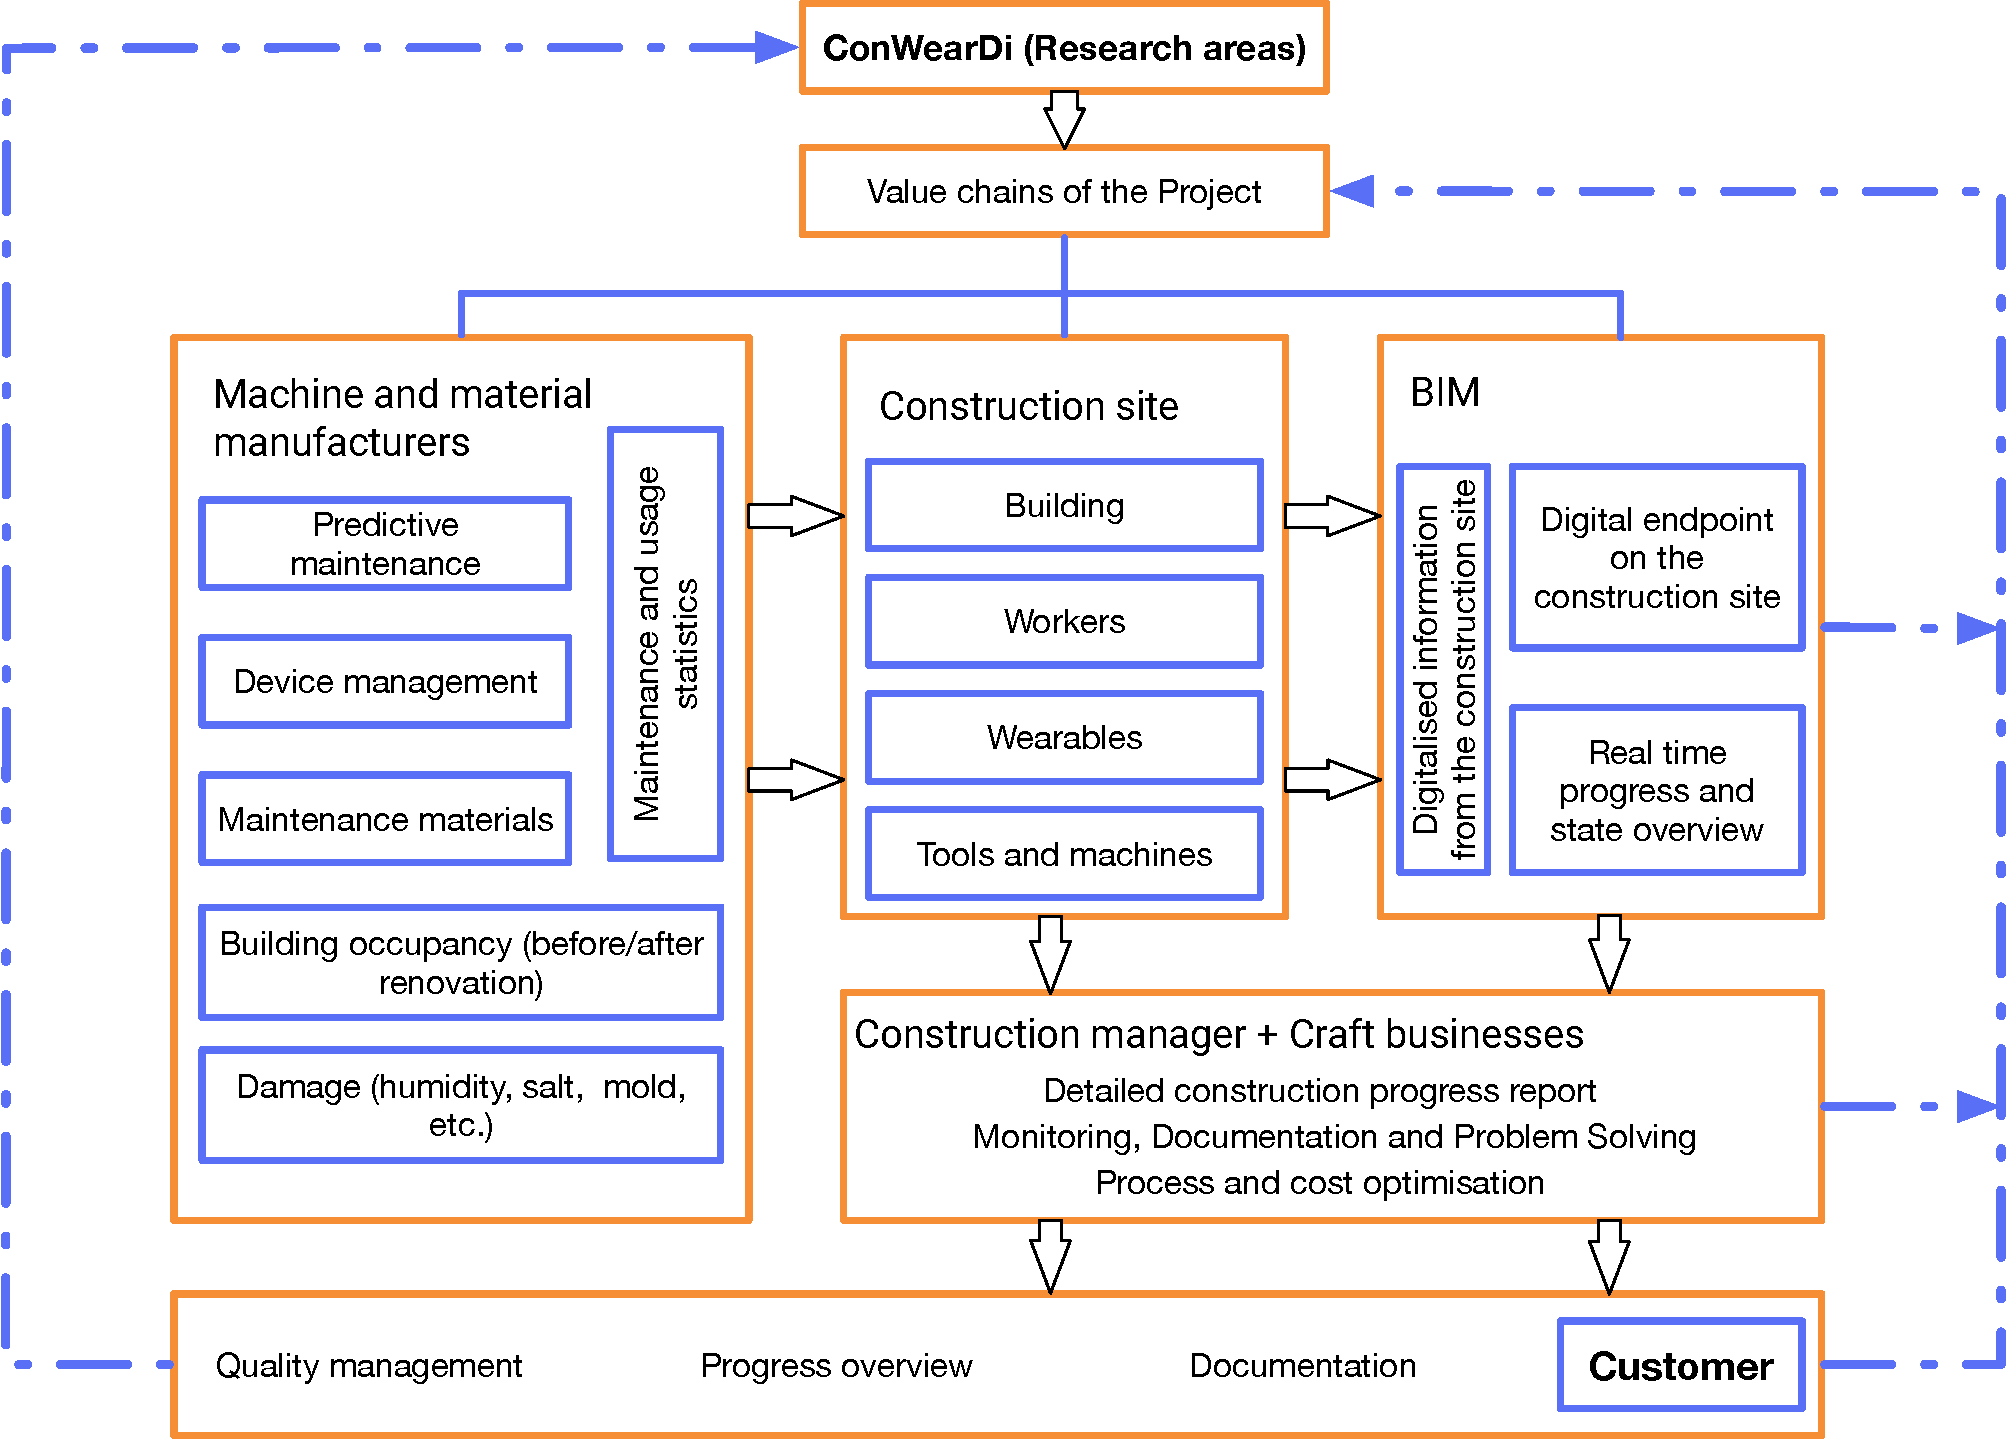
\includegraphics[width=0.7\textwidth]{figures/conweardi-functional}
\caption{Functional graph}
\end{figure*}





\subsection{Theorem-like Constructs}

Other common constructs that may occur in your article are the forms
for logical constructs like theorems, axioms, corollaries and proofs.
ACM uses two types of these constructs:  theorem-like and
definition-like.

Here is a theorem:
\begin{theorem}
  Let $f$ be continuous on $[a,b]$.  If $G$ is
  an antiderivative for $f$ on $[a,b]$, then
  \begin{displaymath}
    \int^b_af(t)\,dt = G(b) - G(a).
  \end{displaymath}
\end{theorem}

Here is a definition:
\begin{definition}
  If $z$ is irrational, then by $e^z$ we mean the
  unique number that has
  logarithm $z$:
  \begin{displaymath}
    \log e^z = z.
  \end{displaymath}
\end{definition}

The pre-defined theorem-like constructs are \textbf{theorem},
\textbf{conjecture}, \textbf{proposition}, \textbf{lemma} and
\textbf{corollary}.  The pre-defined de\-fi\-ni\-ti\-on-like constructs are
\textbf{example} and \textbf{definition}.  You can add your own
constructs using the \textsl{amsthm} interface~\cite{Amsthm15}.  The
styles used in the \verb|\theoremstyle| command are \textbf{acmplain}
and \textbf{acmdefinition}.

Another construct is \textbf{proof}, for example,

\begin{proof}
  Suppose on the contrary there exists a real number $L$ such that
  \begin{displaymath}
    \lim_{x\rightarrow\infty} \frac{f(x)}{g(x)} = L.
  \end{displaymath}
  Then
  \begin{displaymath}
    l=\lim_{x\rightarrow c} f(x)
    = \lim_{x\rightarrow c}
    \left[ g{x} \cdot \frac{f(x)}{g(x)} \right ]
    = \lim_{x\rightarrow c} g(x) \cdot \lim_{x\rightarrow c}
    \frac{f(x)}{g(x)} = 0\cdot L = 0,
  \end{displaymath}
  which contradicts our assumption that $l\neq 0$.
\end{proof}

\section{Conclusions}
This paragraph will end the body of this sample document.
Remember that you might still have Acknowledgments or
Appendices; brief samples of these
follow.  There is still the Bibliography to deal with; and
we will make a disclaimer about that here: with the exception
of the reference to the \LaTeX\ book, the citations in
this paper are to articles which have nothing to
do with the present subject and are used as
examples only.
%\end{document}  % This is where a 'short' article might terminate



\appendix
%Appendix A
\section{Headings in Appendices}
The rules about hierarchical headings discussed above for
the body of the article are different in the appendices.
In the \textbf{appendix} environment, the command
\textbf{section} is used to
indicate the start of each Appendix, with alphabetic order
designation (i.e., the first is A, the second B, etc.) and
a title (if you include one).  So, if you need
hierarchical structure
\textit{within} an Appendix, start with \textbf{subsection} as the
highest level. Here is an outline of the body of this
document in Appendix-appropriate form:
\subsection{Introduction}
\subsection{The Body of the Paper}
\subsubsection{Type Changes and  Special Characters}
\subsubsection{Math Equations}
\paragraph{Inline (In-text) Equations}
\paragraph{Display Equations}
\subsubsection{Citations}
\subsubsection{Tables}
\subsubsection{Figures}
\subsubsection{Theorem-like Constructs}
\subsubsection*{A Caveat for the \TeX\ Expert}
\subsection{Conclusions}
\subsection{References}
Generated by bibtex from your \texttt{.bib} file.  Run latex,
then bibtex, then latex twice (to resolve references)
to create the \texttt{.bbl} file.  Insert that \texttt{.bbl}
file into the \texttt{.tex} source file and comment out
the command \texttt{{\char'134}thebibliography}.
% This next section command marks the start of
% Appendix B, and does not continue the present hierarchy
\section{More Help for the Hardy}

Of course, reading the source code is always useful.  The file
\path{acmart.pdf} contains both the user guide and the commented
code.

\begin{acks}
  The authors would like to thank Dr. Yuhua Li for providing the
  MATLAB code of the \textit{BEPS} method.

  The authors would also like to thank the anonymous referees for
  their valuable comments and helpful suggestions. The work is
  supported by the \grantsponsor{GS501100001809}{National Natural
    Science Foundation of
    China}{http://dx.doi.org/10.13039/501100001809} under Grant
  No.:~\grantnum{GS501100001809}{61273304}
  and~\grantnum[http://www.nnsf.cn/youngscientists]{GS501100001809}{Young
    Scientists' Support Program}.

\end{acks}
